\chapter{Derivatives (1)}
\label{ch:derivs1}
To work with derivatives we first have to know what a limit is, but to motivate
why we are going to study limits we essentially need to explain what a
derivative is.  In order to resolve this potentially circular logic, we will
first motivate the idea of a derivative in this short chapter, then discuss how
to compute limits in detail in the next chapter, and then we will return and
discuss derivatives armed with a better understanding of limits.


% added explanation of why this chapter exists


Let's first look at the two classical problems that gave rise to the notion of a
derivative: finding the equation of the line tangent to a curve at a point, and
finding the instantaneous velocity of a moving object.

\section{The tangent line to a curve} 
\label{sec:tangent} Suppose you have a function $y=f(x)$ and you draw its graph.
If you want to find the tangent line to the graph of $f$ at some given point on the
graph of $f$, how would you do that?
% A better explanation of what a tangent line even is, should be put here
\begin{figure}[h]\centering
  
    \begin{picture} (270.000000,270.000000)(0,0)
    \put(0.0, 0.0){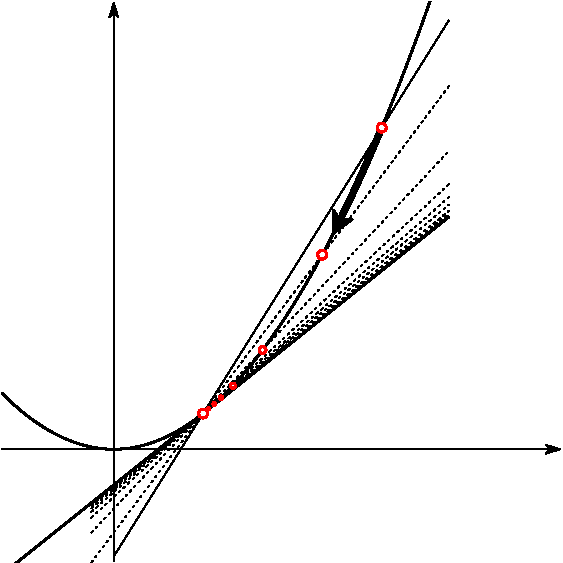
\includegraphics{02constructingTheTangent.pdf}}
        \put( 95.48,  71.75){\sffamily\itshape \makebox[0pt][r]{$P$}}
    \put(181.24, 208.97){\sffamily\itshape \makebox[0pt][r]{$Q$}}
    \put(217.40, 166.09){\sffamily\itshape tangent}
    \put(217.40, 260.42){\sffamily\itshape a secant}
\end{picture}

  \caption{Constructing the tangent by letting $Q\to P$}
  \label{fig:constructTheTangent}
\end{figure}

Let $P$ be the point on the graph at which want to draw the tangent.  If you are
making a real paper and ink drawing you would take a ruler, make sure it goes
through $P$, and then turn it until it doesn't cross the graph anywhere else (at
least, nowhere else near $P$).

If you are using equations to describe the curve and lines, then you
could pick a point $Q$ on the graph and construct the line through $P$
and $Q$ (``construct'' means ``find an equation for'').  This line is
called a ``secant line'', and it won't precisely be the tangent line, but if you
choose $Q$ to be very close to $P$ then the secant line will be close to the
tangent line.

So this is our recipe for constructing the tangent through $P$: pick another
point $Q$ on the graph, find the line through $P$ and $Q$, and see what happens
to this line as you take $Q$ closer and closer to $P$.  The resulting secants
will then get closer and closer to some line, and that line is the tangent.

We'll write this in formulas in a moment, but first let's worry about
how close $Q$ should be to $P$.  We can't set $Q$ equal to $P$,
because then $P$ and $Q$ don't determine a line, since we need \emph{two}
points to determine a line.  If we choose $Q$ different from $P$
then we won't get the tangent, but at best something that is
``close'' to it.  Some people have suggested that one should take $Q$
``infinitely close'' to $P$, but it isn't clear what that would mean.
The concept of a limit is needed to clarify this issue.

\section{An example -- tangent to a parabola} 
\label{sec:tangent-to-parabola}
To make things more concrete, let us take the function $f(x)=x^2$, and attempt
to find the equation of the tangent line to $y=f(x)$ at the point $P=(1, 1)$.
The graph of $f$ is of course a parabola.

Any line through the point $P(1,1)$ has equation
\[
y-1 = m(x-1)
\]
where $m$ is the slope of the line.  So instead of finding the equations of the
secant and tangent lines, we can simply find their slopes.

\begin{center}
  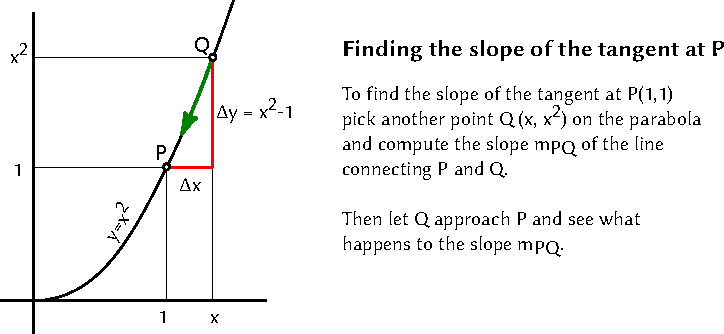
\includegraphics[width=0.7\textwidth]{02DeltaxDeltay.pdf}
\end{center}

Let $Q$ be the other point on the parabola, with coordinates $(x, x^2)$.  We can ``move
$Q$ around on the graph'' by changing $x$, although we are not allowed to set
$x=1$ because $P$ and $Q$ have to be different points.  By the ``rise over run''
formula, the slope of the secant line joining $P$ and $Q$ is
\[
  m_{PQ}= \frac{\Delta y}{\Delta x}
  \quad\text{where}\quad
  \Delta y=x^2-1
  \quad\text{and}\quad
  \Delta x = x-1.
\]
By factoring $x^2-1$ we can rewrite the formula for the slope as follows
\begin{equation}\label{eq:secant-slope-simplified}
  m_{PQ}= \frac{\Delta y}{\Delta x}
  =\frac{x^2-1}{x-1}
  =\frac{(x-1)(x+1)}{x-1}
  = x+1.
\end{equation}
As $x$ gets closer to $1$, the slope $m_{PQ}$, being $x+1$, gets closer to the
value $1+1= 2$.  We say that
\begin{equation*}
  \textit{the limit of the slope $m_{PQ}$ as $Q$ approaches $P$ is $2$.}
\end{equation*}
In symbols,
\[
\lim_{Q\to P} m_{PQ} = 2,
\]
or, since $Q$ approaching $P$ is the same as $x$ approaching 1,
\begin{equation}\label{eq:tangent-slope-found}
  \lim_{x\to 1} m_{PQ} = 2.
\end{equation}
So we find that the tangent line to the parabola $y=x^2$ at the point $(1,1)$ has equation
\[
y-1 = 2 (x-1), \text{~i.e.~} y=2x-1.
\]
A warning: we cannot substitute $x=1$ in equation
\eqref{eq:secant-slope-simplified} to get \eqref{eq:tangent-slope-found}, even
though it looks like that's what we did.  The reason why we can't do that is
that when $x=1$ the point $Q$ coincides with the point $P$ so ``the line through
$P$ and $Q$'' is not defined; also, if $x=1$ then $\Delta x=\Delta y =0$ so that
the rise-over-run formula for the slope gives
\[
m_{PQ} = \frac{\Delta y}{\Delta x} = \frac 00 = \text{~undefined.}
\]
It is only after the algebra trick in \eqref{eq:secant-slope-simplified} that
setting $x=1$ gives something that is well-defined.  But if the intermediate
steps leading to $m_{PQ}=x+1$ aren't valid for $x=1$, why should the final
result mean anything for $x=1$?

We did something more complicated than just setting $x=1$: we did a calculation
which is valid for all $x\neq 1$, and later looked at what happens if $x$ gets
``very close to 1.''  This is the essence of a limit, and we'll study these
ideas in detail soon.


\section{Instantaneous velocity} 
When you are riding in a car, the speedometer tells you how fast you are going,
i.e.\ what your velocity is.  But what exactly does it mean when the speedometer
says your car is traveling at a speed of (say) 50 miles per hour?

\smallskip

\begin{figure}[h]
  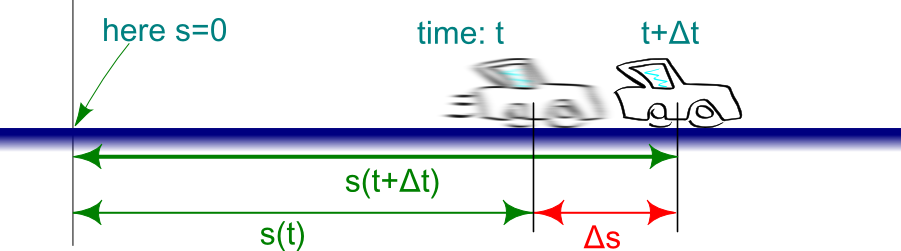
\includegraphics[width=0.6\textwidth]{02car.png}
  %\centering \input ../figures/221/02car.tex
\end{figure}

\smallskip

We all know what \emph{average velocity} is.  Namely, if it takes you two hours
to cover 100 miles, then your average velocity was
\[
\frac{\text{distance traveled}}{\text{time it took}} = 50 \text{ miles per
  hour}.
\]
This is not the number the speedometer provides you -- it doesn't wait two
hours, measure how far you went, and then compute
$\text{distance}/\text{time}$. If the speedometer in your car tells you that you
are driving 50mph, then that should be your velocity \emph{at the moment} that
you look at your speedometer, i.e.\ ``distance traveled over time it took'' at
the moment you look at the speedometer.  But during the moment you look at your
speedometer no time goes by (because a moment has no length) and you didn't
cover any distance, so your velocity at that moment is $\frac00$, which is
undefined.  Your velocity at \emph{any} moment is undefined.  But then what is
the speedometer telling you?

To put all this into formulas we need to introduce some notation.  Let $t$ be
the time (in hours) that has passed since we got onto the road, and let $s(t)$
be our distance from our starting point (in miles).

Instead of trying to find the velocity exactly at time $t$, we find a formula
for the average velocity during some (short) time interval beginning at time
$t$.  We'll write $\Delta t$ for the length of the time interval.

At time $t$ we are $s(t)$ miles from our start.  A little later, at time
$t+\Delta t$ we are $s(t+\Delta t)$ miles from our start.  Therefore, during the
time interval from $t$ to $t+\Delta t$, we have moved
\[
s(t+\Delta t) - s(t)\text{ miles,}
\]
and therefore our average velocity in that time interval was
\[
\frac{s(t+\Delta t) - s(t)}{\Delta t} \text{~ miles per hour.}
\]
The shorter we make the time interval (the smaller we choose $\Delta t$) the
closer this number should be to the instantaneous velocity at time $t$.

So we have the following formula (definition, really) for the velocity at time
$t$
\begin{equation}
  v(t) = \lim_{\Delta t\to0} \frac{s(t+\Delta t)- s(t)}{\Delta t}.
\end{equation}

\section{Rates of change} 
\label{sec:rates-of-change} The two previous examples have much in common.  If
we ignore all the details about geometry, graphs, highways and motion, the
following happened in both examples:

We had a function $y=f(x)$, and we wanted to know how much $f(x)$ changes if $x$
changes.  If we change $x$ to $x+\Delta x$, then $y$ will change from $f(x)$ to
$f(x+\Delta x)$.  The change in $y$ is therefore
\[
\Delta y = f(x+\Delta x) - f(x),
\]
and the average rate of change is
\begin{equation} \label{eq:difference-quotient} \frac{\Delta y}{\Delta x} =
  \frac{f(x+\Delta x) - f(x)}{\Delta x}.
\end{equation}
This is the average rate of change of $f$ over the interval from $x$ to
$x+\Delta x$.  To define \emph{the rate of change of the function $f$ at $x$} we
let the length $\Delta x$ of the interval become smaller and smaller, in the
hope that the average rate of change over the shorter and shorter time intervals
will get closer and closer to some number.  If that happens then that ``limiting
number'' is called the rate of change of $f$ at $x$, or, the \emph{derivative}
of $f$ at $x$.  It is written as
\begin{equation}
  \label{eq:derivative-defined-first-time}
  f'(x) = \lim_{\Delta x\to 0}\frac{f(x+\Delta x) - f(x)}{\Delta x}.
\end{equation}
Derivatives and what we can do with them are what the first portion of this
course is about.  The description we just went through shows that to understand
what a derivative is, we need to understand more about this ``limiting process''
so that we can have a concrete understanding of statements like
\eqref{eq:derivative-defined-first-time}.

\section{Examples of rates of change} 

\subsection{Acceleration as the rate at which velocity changes} 
As you are driving in your car your velocity may change over time.  Suppose
$v(t)$ is your velocity at time $t$ (measured in miles per hour).  You could try
to figure out how fast your velocity is changing by measuring it at one moment
in time (you get $v(t)$), then measuring it a little later (you get $v(t+\Delta
t)$)).  You conclude that your velocity increased by $\Delta v = v(t+ \Delta t)
- v(t)$ during a time interval of length $\Delta t$, and hence
\begin{multline*}
  \left\{
    \parbox{7em}{\centering average rate at which your velocity changed}
  \right\}
  = \frac{\text{change in velocity}}{\text{duration of time interval}}
  =\frac{\Delta v}{\Delta t} =\frac{v(t+ \Delta t) - v(t)}{\Delta t}.
\end{multline*}
This rate of change is called your \textit{average acceleration} (over the time
interval from $t$ to $t+\Delta t$).  Your \textit{instantaneous acceleration} at
time $t$ is the limit of your average acceleration as you make the time interval
shorter and shorter:
\[
\left\{ \text{acceleration at time $t$} \right\} = a = \lim_{\Delta t\to 0}
\frac{v(t+ \Delta t) - v(t)}{\Delta t}.
\]
The average and instantaneous accelerations are measured in ``miles per hour per
hour'':
\[
(\textrm{mi}/\textrm{h})/\textrm{h} = \textrm{mi}/\textrm{h}^2.
\]
Or, if you had measured distances in \textit{meters} and time in
\textit{seconds} then velocities would be measured in \textit{meters per
  second}, and acceleration in \textit{meters per second per second}, which is
the same as meters per second$^2$: ``meters per squared second''.




\subsection{Reaction rates} 
Imagine a chemical reaction in which two substances A and B react in such a way
that A converts B into A.  The reaction could proceed by
\[
\textrm{A} +  \textrm{B} \longrightarrow 2\textrm{A}.
\]
If the reaction is taking place in a closed reactor, then the ``amounts'' of A
and B will change with time.  The amount of B will decrease, while the amount of
A will increase.  Chemists write $[\textrm{A}]$ for the concentration of ``A''
in the chemical reactor (measured in moles per liter).  We're mathematicians so
we will write ``$[\textrm{A}](t)$'' for the concentration of A present at time
$t$.
\begin{figure}[h]
  \begin{center}
    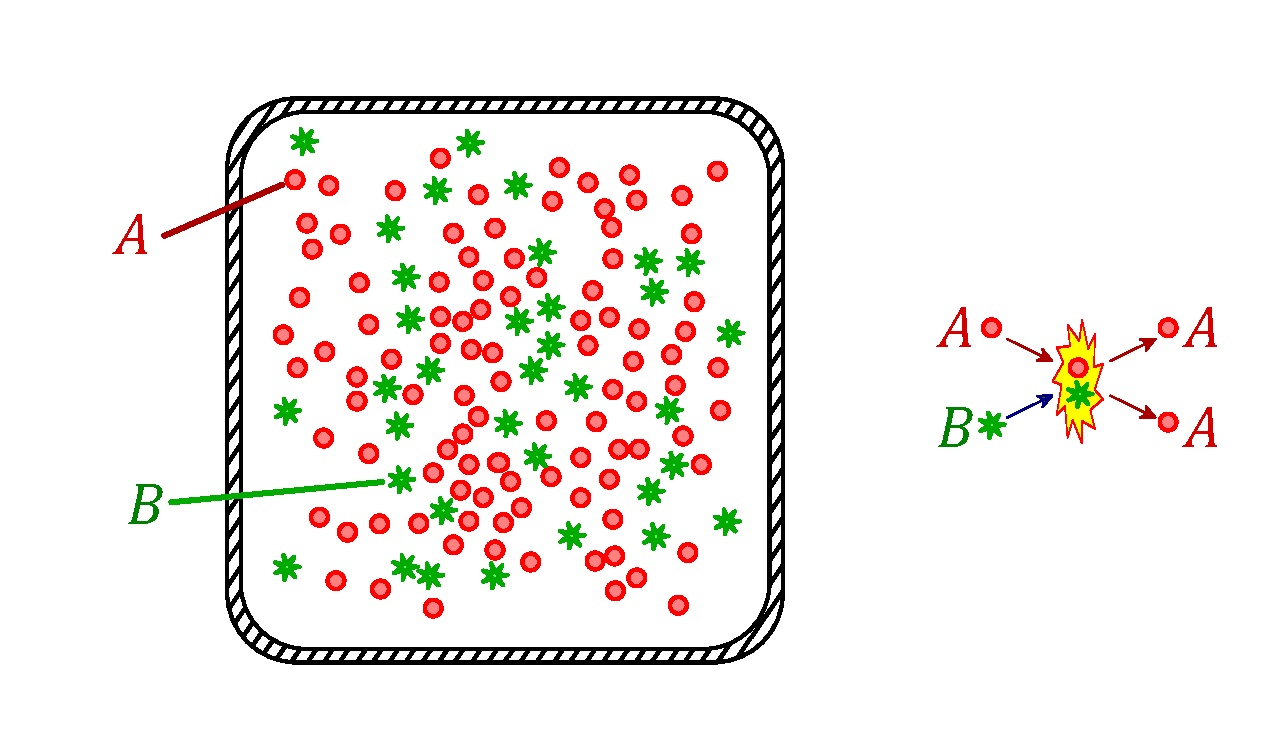
\includegraphics[width=0.6\textwidth]{02ABreaction.pdf}
  \end{center}
  \caption{A chemical reaction in which A converts B into A.}
  \label{fig:02ABreaction}
\end{figure}

To describe how fast the amount of A is changing we consider the derivative
of $[\textrm{A}]$ with respect to time:
\[
[A]'(t)= \lim_{\Delta t\to 0}
\frac {[\textrm{A}](t+\Delta t) - [\textrm{A}](t)}  {\Delta t}.
\]
This quantity is the rate of change of [A].  In chemistry and physics, it is
more common to write the derivative in \textsc{Leibniz} notation:
\[
\frac{d[\textrm{A}]}{dt}.
\]

\textit{How fast does the reaction take place?}  If you add more A or more B to
the reactor then you would expect that the reaction would go faster (i.e., that
more A would be produced per second).  The law of \textit{mass-action kinetics}
from chemistry states this more precisely. For our particular reaction it would
say that the rate at which A is consumed is given by
\[
\frac{d[\textrm{A}]}{dt} = k \, [\textrm{A}] \, [\textrm{B}],
\]
where the constant $k$ is called the \textit{reaction constant}, which you could
measure by timing how fast the reaction goes.

\section{Problems} 
\problemfont% 
\begin{multicols}{2}\setlength{\parindent}{0pt}
\problem \label{ex:02derivATonethird} 
Repeat the reasoning in \S\ref{sec:tangent-to-parabola} to find the slope of the
tangent line at the point $(\frac13, \frac19)$, or more generally at any point
$(a, a^2)$ on the parabola with equation $y=x^2$.

\problem Repeat the reasoning in \S\ref{sec:tangent-to-parabola} to find the 
slope of the tangent line at the point $(\frac12, \frac18)$, or more generally
at any point $(a, a^3)$ on the curve with equation $y=x^3$.

\problem Simplify the algebraic expressions you get when you compute $\Delta y$ and 
$\Delta y/\Delta x$ for the following functions
\begin{align*}
  (a)~& y = x^2-2x+1 \\
  (b)~& y = \frac1x \\
  (c)~& y = 2^x
  \end{align*}
\answer 
\textbf{(a)}
\begin{align*}
  \Delta y &= (x+\Delta x)^2  -2 (x+\Delta x)+1 - [x^2-2x+1]\\
  &=(2x-2)\Delta x +(\Delta x)^2 \text{ so that}\\
  \frac{\Delta y}{\Delta x}&= 2x-2 + \Delta x
\end{align*}
\endanswer

\problem This figure shows a plot of the distance traveled $s(t)$ (in miles)
versus time $t$ (in minutes):
\smallskip

\centerline{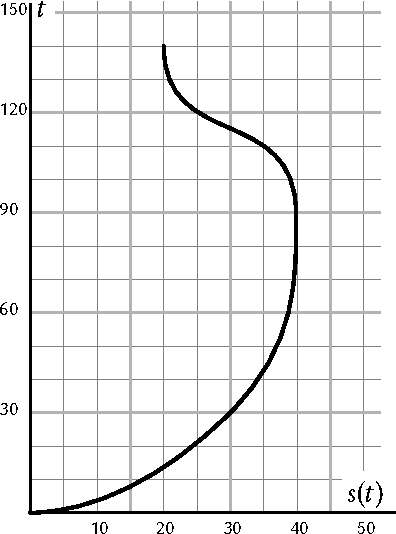
\includegraphics[width=0.4\textwidth]{02velocityproblem.pdf}}

\subprob Something is wrong:  the curve in the graph obviously doesn't pass the vertical
line test, so it cannot be the graph of a function.  How can it be the graph of $s(t)$
versus $t$?
% This problem statement is incredibly misleading ("graph of a function").
\answer 
In this picture $s(t)$ is on the horizontal axis and $t$ is on the vertical axis, so
horizontal and vertical have been swapped. This curve should pass the \emph{horizontal
line test}, which it does.
\endanswer

\subprob Use the plot to estimate the instantaneous
velocity at the following times
\begin{center}
  \begin{tabular}{cp{1in}}
    \toprule
    $t$ (min) &\hfill $v(t)$ \\[1pt]
    \midrule
    30 & \\[1pt]
    \midrule
    60 & \\[1pt]
    \midrule
    90 & \\[1pt]
    \midrule
    120 & \\
    \bottomrule
  \end{tabular}
\end{center}
Describe in one or two short sentences what you did to find
your estimates.
\answer 
With a ruler I tried to draw the closest tangent lines at
the four different times.  Then I measured the slope of those
four lines using the grid.
\endanswer

\subprob Make a graph of the instantaneous velocity $v(t)$.

\problem Look ahead at Figure~\ref{fig:03backwardCosSandwich} in the next 
chapter.  What is the derivative of $f(x) = x\cos\frac\pi x$ at the
points $A$ and $B$ on the graph?
\answer 
At $A$ and $B$ the graph of $f$ is tangent to the drawn lines, so
the derivative at $A$ is $-1$ and ther derivative at $B$ is $+1$.
\endanswer
  
\problem Suppose that some quantity $y$ is a function of some other quantity 
$x$, and suppose that $y$ is a mass (measured in pounds)
and $x$ is a length (measured in feet).  What units do the increments
$\Delta y$ and $\Delta x$, and the derivative $ dy/d x$, have?
\answer 
$\Delta x$ : feet.  $\Delta y$ pounds. $\frac{\Delta y}{\Delta x}$
and $\frac{dy}{dx}$ are measured in pounds per feet.
\endanswer

\problem A tank is filling with water.  The volume (in gallons) of water in 
the tank at time $t$ (seconds) is $V(t)$.  What units does the
derivative $V'(t)$ have?
\answer 
Gallons per second.
\endanswer

\problem \groupproblem Let $A(x)$ be the area of an equilateral triangle whose
sides measure $x$ inches.
% This problem is not appropriate for this chapter, where derivatives have not
% even been defined.

\subprob Show that $\frac{dA}{dx}$ has the units of a length.

\subprob Which length does $\frac{dA}{dx}$ represent geometrically?  [Hint: draw
two equilateral triangles, one with side $x$ and another with side $x+\Delta x$.
Arrange the triangles so that they both have the origin as their lower left hand
corner, and so their bases are on the x-axis.]

\answer 
(a) $A(x)$ is an area so it has units square inch and $x$ is
measured in inches, so $\dfrac{dA}{dx}$ is measured in
$\displaystyle\frac{\text{inch}^2}{\text{inch}} = \text{inch}$.

\input ../figures/221/02triangleareagrowth.tex

(b) Hint: The extra area $\Delta A$ that you get when the side of
an equilateral triangle grows from $x$ to $x+\Delta x$ can be
split into a thin parallelogram and a very tiny triangle.  Ignore
the area of the tiny triangle since the area of the parallelogram
will be much larger.  What is the area of this parallelogram?




The area of a parallelogram is ``base time height'' so here it is
$h\times\Delta x$, where $h$ is the height of the triangle.




Conclusion: $\displaystyle \frac{\Delta A}{\Delta x}
\approx\frac{h\Delta x}{\Delta x} = h$.




The derivative is therefore the height of the triangle.




\endanswer








\problem \groupproblem Let $A(x)$ be the area of a square with 
side $x$, and let $L(x)$ be
the perimeter of the square (sum of the lengths of all its sides).
Using the familiar formulas for $A(x)$ and $L(x)$ show that $A'(x) =
\frac12 L(x)$.
% This problem is not appropriate for this chapter, where derivatives have not even been defined.


Give a geometric interpretation that explains why $\Delta A \approx
\frac12 L(x) \Delta x$ for small $\Delta x$.








\problem Let $A(r)$ be the area enclosed by a circle of radius $r$, and let 
$L(r)$ be the circumference of the circle.  Show that $ A'(r) = L(r) $.
(Use the familiar formulas from geometry for the area and circumference
of a circle.)
% This problem is not appropriate for this chapter, where derivatives have not even been defined.






\problem Let $V(r)$ be the volume enclosed by a sphere of radius $r$, and let 
$S(r)$ be the its surface area.
% This problem is not appropriate for this chapter, where derivatives have not even been defined.


\subprob Show that $V'(r) = S(r)$.  (Use the
formulas $V(r) = \frac43\pi r^3$ and $S(r) = 4\pi r^2$.)




\subprob Give a geometric explanation of the fact that
$\frac{dV} {dr} = S$.




[Hint: to visualize what happens to the volume of a sphere when
you increase the radius by a very small amount, imagine  the sphere is
the Earth, and you increase the radius by covering the Earth with
a layer of water that is 1 inch deep.  How much does the volume
increase?  What if the depth of the layer was ``$\Delta r$''?]




\problem \label{ex:bad-calculator-bad} \groupproblem 
\itshape Should you trust your calculator?\upshape




Find the slope of the tangent to the parabola
\[
y=x^2
\]
at the point
$(\frac13, \frac{1}{9})$ (You have already done this: see exercise
\ref{ex:02derivATonethird}).




Instead of doing the algebra you could try to compute the slope by
using a calculator.  This exercise is about how you do that and what
happens if you try (too hard).




Compute $\frac{\Delta y}{\Delta x}$ for various values of $\Delta x$:
\[
\Delta x = 0.1, 0.01, 0.001, 10^{-6}, 10^{-12}.
\]
As you choose $\Delta x$ smaller your computed $\frac{\Delta
  y}{\Delta x}$ ought to get closer to the actual slope.  Use at
least 10 decimals and organize your results in a table like this:
Look carefully at the ratios $\Delta y/\Delta x$.  Do they look like
they are converging to some number?  Compare the values of
$\frac{\Delta y}{\Delta x}$ with the true value you got in the
beginning of this problem.












\end{multicols}
\noproblemfont




\begin{table}[h]
  \centering
  \begin{tabular}{r|p{75pt}|p{75pt}|p{75pt}|p{75pt}}
    \hline\rule[-6pt]{0pt}{18pt}
    $\Delta x$ & $a+\Delta x$ & $f(a+\Delta x)$ & $\Delta y$ & $\Delta y / \Delta x$ \\
    \hline\rule[-6pt]{0pt}{18pt}
    \texttt{0.1} &&&&\\
    \hline\rule[-6pt]{0pt}{18pt}
    \texttt{0.01} &&&&\\
    \hline\rule[-6pt]{0pt}{18pt}
    \texttt{0.001} &&&&\\
    \hline\rule[-6pt]{0pt}{18pt}
    \texttt{10}$^{\texttt{-6}}$ &&&&\\
    \hline\rule[-6pt]{0pt}{18pt}
    \texttt{10}$^{\texttt{-12}}$ &&&&\\
    \hline
  \end{tabular}
  \medskip
  
  \caption{The table for Problem~\ref{ex:bad-calculator-bad}.
  Approximate the derivative of $f(x) = x^2$ at
  $a=1/3 \approx 0.333\,333\,333\,333$ by computing $\bigl(f(a+\Delta
  x) - f(a)\bigr)/\Delta x$ for smaller and smaller values of $\Delta
  x$.  You know from Problem~\ref{ex:02derivATonethird} that
  the derivative is $f'(a) = 2a = 2/3$.  Which value of
  $\Delta x$ above gives you the most accurate answer?}
\end{table}


%%% Local Variables:
%%% mode: latex
%%% TeX-master: "free221"
%%% End:
